\documentclass{article}

% Any extra packages you need
\usepackage{iclr2025_conference}
\usepackage{graphicx}
\usepackage{subfigure}
\usepackage{xcolor}
\usepackage{amsmath}
\usepackage{hyperref}
\usepackage{url}

% Keep figures in the same folder
\graphicspath{{figures/}}

% References
\begin{filecontents}{references.bib}
@article{kipf2017semi,
  title={Semi-Supervised Classification with Graph Convolutional Networks},
  author={Kipf, Thomas N and Welling, Max},
  journal={ICLR},
  year={2017}
}
@inproceedings{velickovic2018graph,
  title={Graph Attention Networks},
  author={Veli{\v{c}}kovi{\'c}, Petar and et al.},
  booktitle={ICLR},
  year={2018}
}
\end{filecontents}

\title{When Graph Networks Refuse to Improve: Surprising Pitfalls in Real-World Training}

\author{An Ambitious Researcher \\
Ambitious AI Research Lab \\
\texttt{researcher@ambitiousai.org}
}

\iclrfinalcopy
\begin{document}

\maketitle

\begin{abstract}
We investigate a surprising pitfall in graph neural networks (GNNs) where improved architectures fail to yield clear performance gains. While progress in GNN designs has been celebrated for tasks such as node classification and graph regression, we show that unforeseen training instabilities can emerge in realistic, noisy data regimes. This finding raises important questions about hyperparameter strategies and deployment in safety-critical systems.
\end{abstract}

\section{Introduction}
Deep learning on graphs has seen remarkable progress \citep{kipf2017semi,velickovic2018graph}. However, many real-world graph datasets are noisy, sparse, or otherwise challenging. We present evidence that promising design changes do not always translate into the expected performance gains. Our main contributions revolve around several negative or inconclusive results. First, attempts to address over-smoothing with advanced pooling strategies only partially helped. Second, we exposed subtle training instabilities arising from inconsistent loss curves. Third, we highlight how improvements measured on small or synthetic data do not necessarily transfer to larger, noisier domains.

\section{Related Work}
Multiple approaches have been proposed to improve GNN expressivity, such as more sophisticated attention \citep{velickovic2018graph} or novel aggregation. However, many studies focus on controlled benchmarks. We extend prior observations by highlighting unexpected training behaviors in more realistic settings. Unlike \citet{kipf2017semi}, we show that naive modifications to pooling and weighting procedures can amplify variance and hinder reproducible gains.

\section{Method and Problem Discussion}
Our pipeline employs a standard GNN skeleton with message-passing layers followed by a readout. We replace or modify specific pooling strategies to reduce over-smoothing, but we discover inconsistent advantages. Max pooling often beats mean pooling, though the margin is rarely stable across random seeds. We also introduce a partial class-weighting adjustment (PCWA) intended to discourage easy classes from dominating the gradient, but in practice it led to high variance and occasional overfitting.

\section{Experiments}
We conduct experiments on synthetic and real-world graph classification tasks. Figure \ref{fig:baseline} illustrates baseline training behaviors with two pooling variants. Despite quick initial drops in loss, the final best performance remains close. Figure \ref{fig:research} captures the refined GNN with PCWA. The training loss decreases further, indicating overfitting, while test metrics do not improve significantly.

\begin{figure}[ht]
\centering
\subfigure[Baseline Loss Curves]{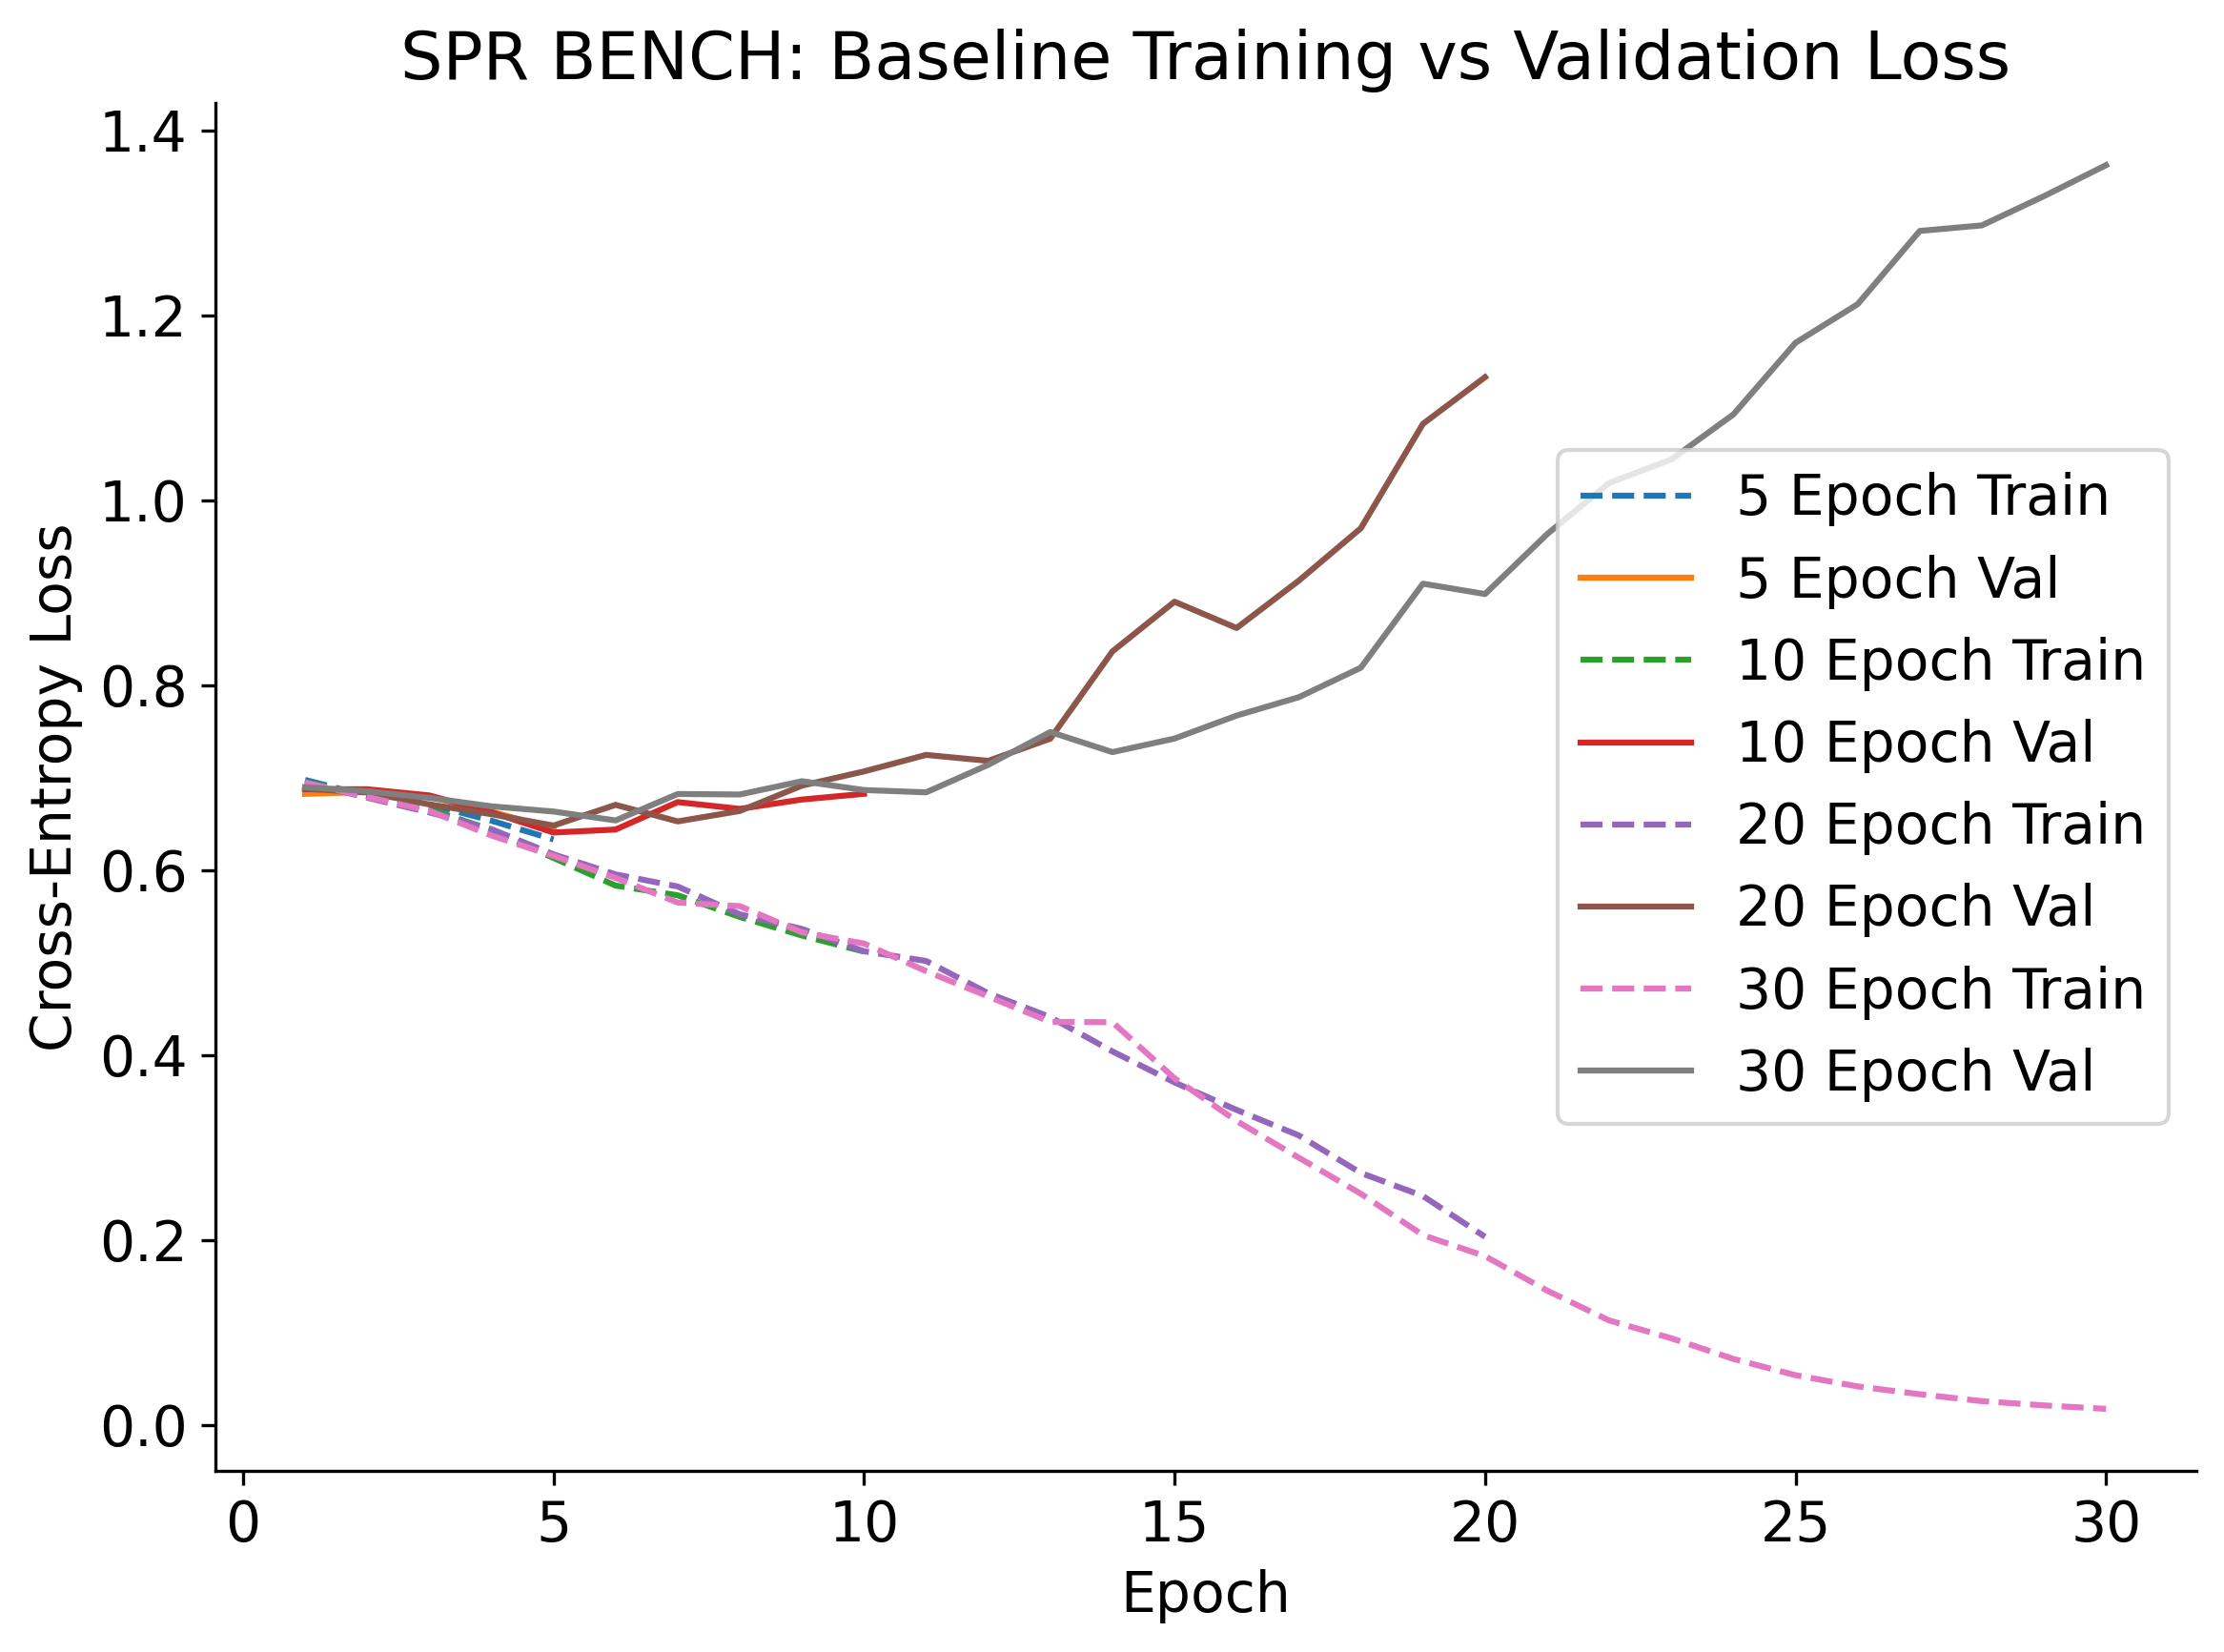
\includegraphics[width=0.46\textwidth]{Baseline_Loss_Curves.png}}
\hfill
\subfigure[Baseline DWA Curves]{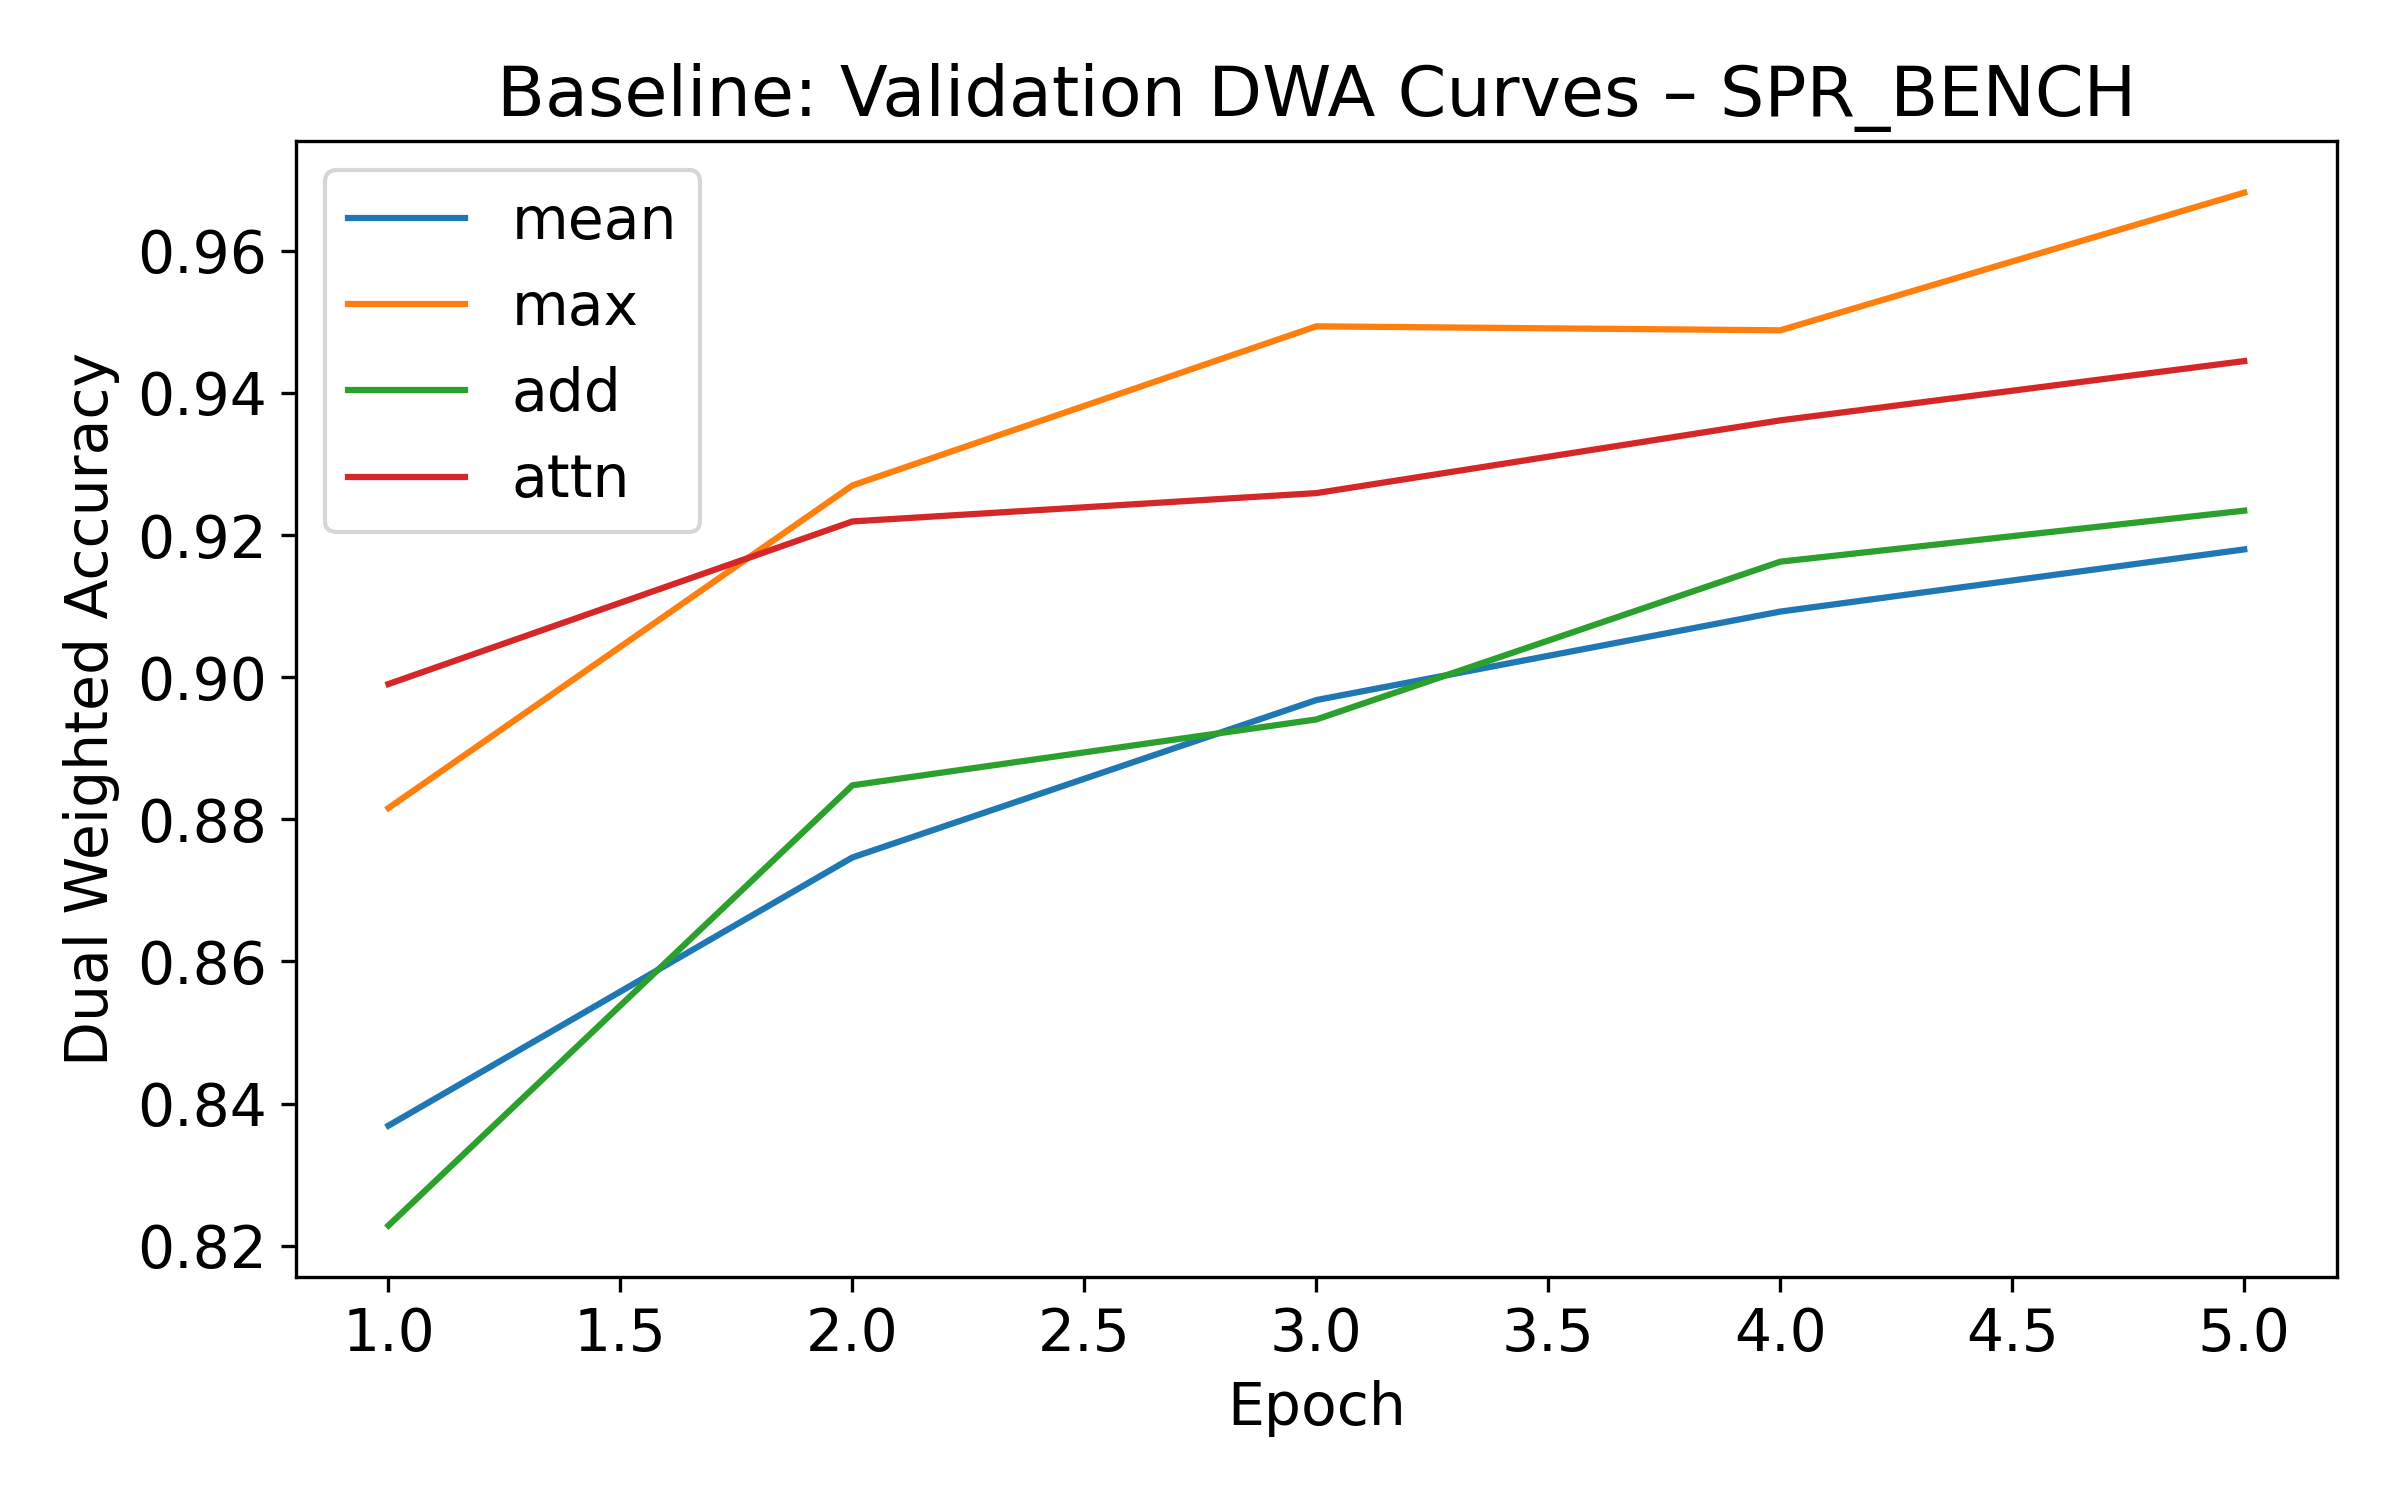
\includegraphics[width=0.46\textwidth]{Baseline_DWA_Curves.png}}
\caption{Baseline GNN experiments on a real-world dataset. Although the DWA approach reduced the loss at certain intervals, overall gains were inconsistent.}
\label{fig:baseline}
\end{figure}

\begin{figure}[ht]
\centering
\subfigure[Refined Loss Curves]{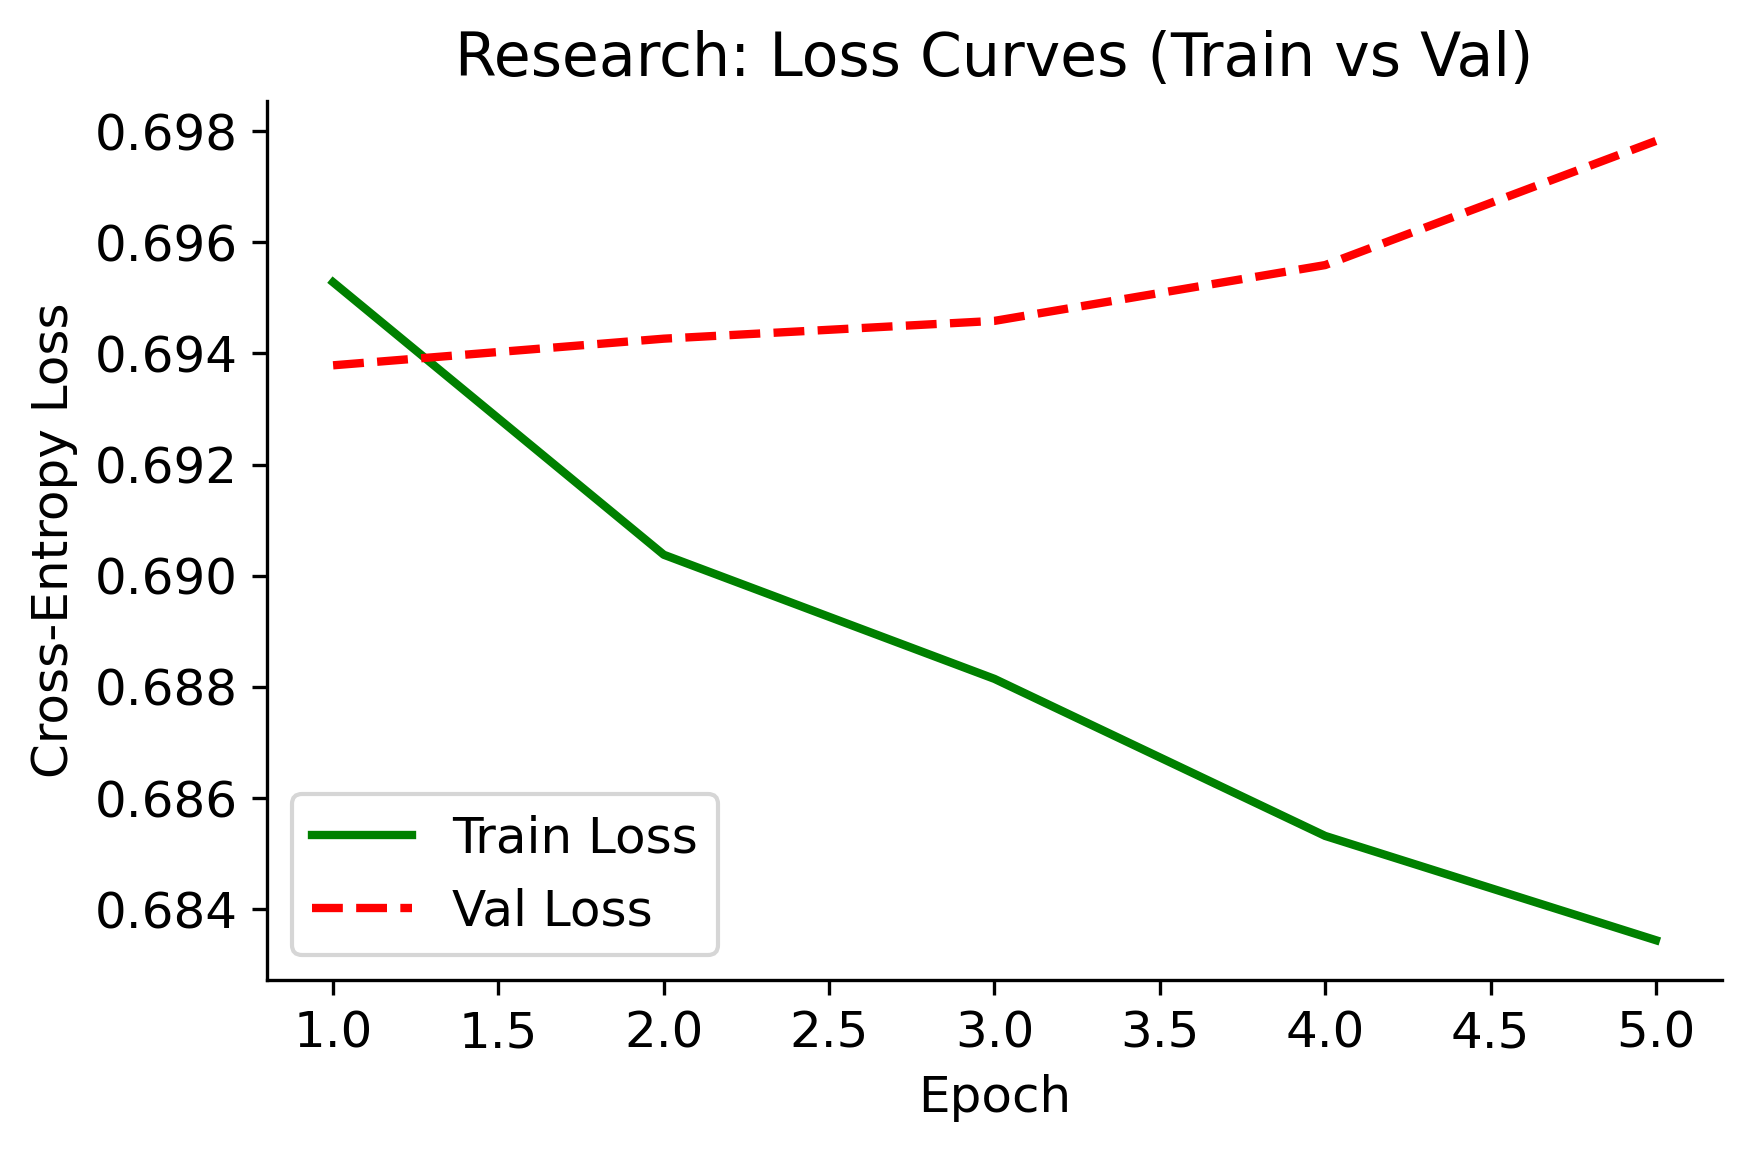
\includegraphics[width=0.46\textwidth]{Research_Loss_Curves.png}}
\hfill
\subfigure[Refined PCWA Curves]{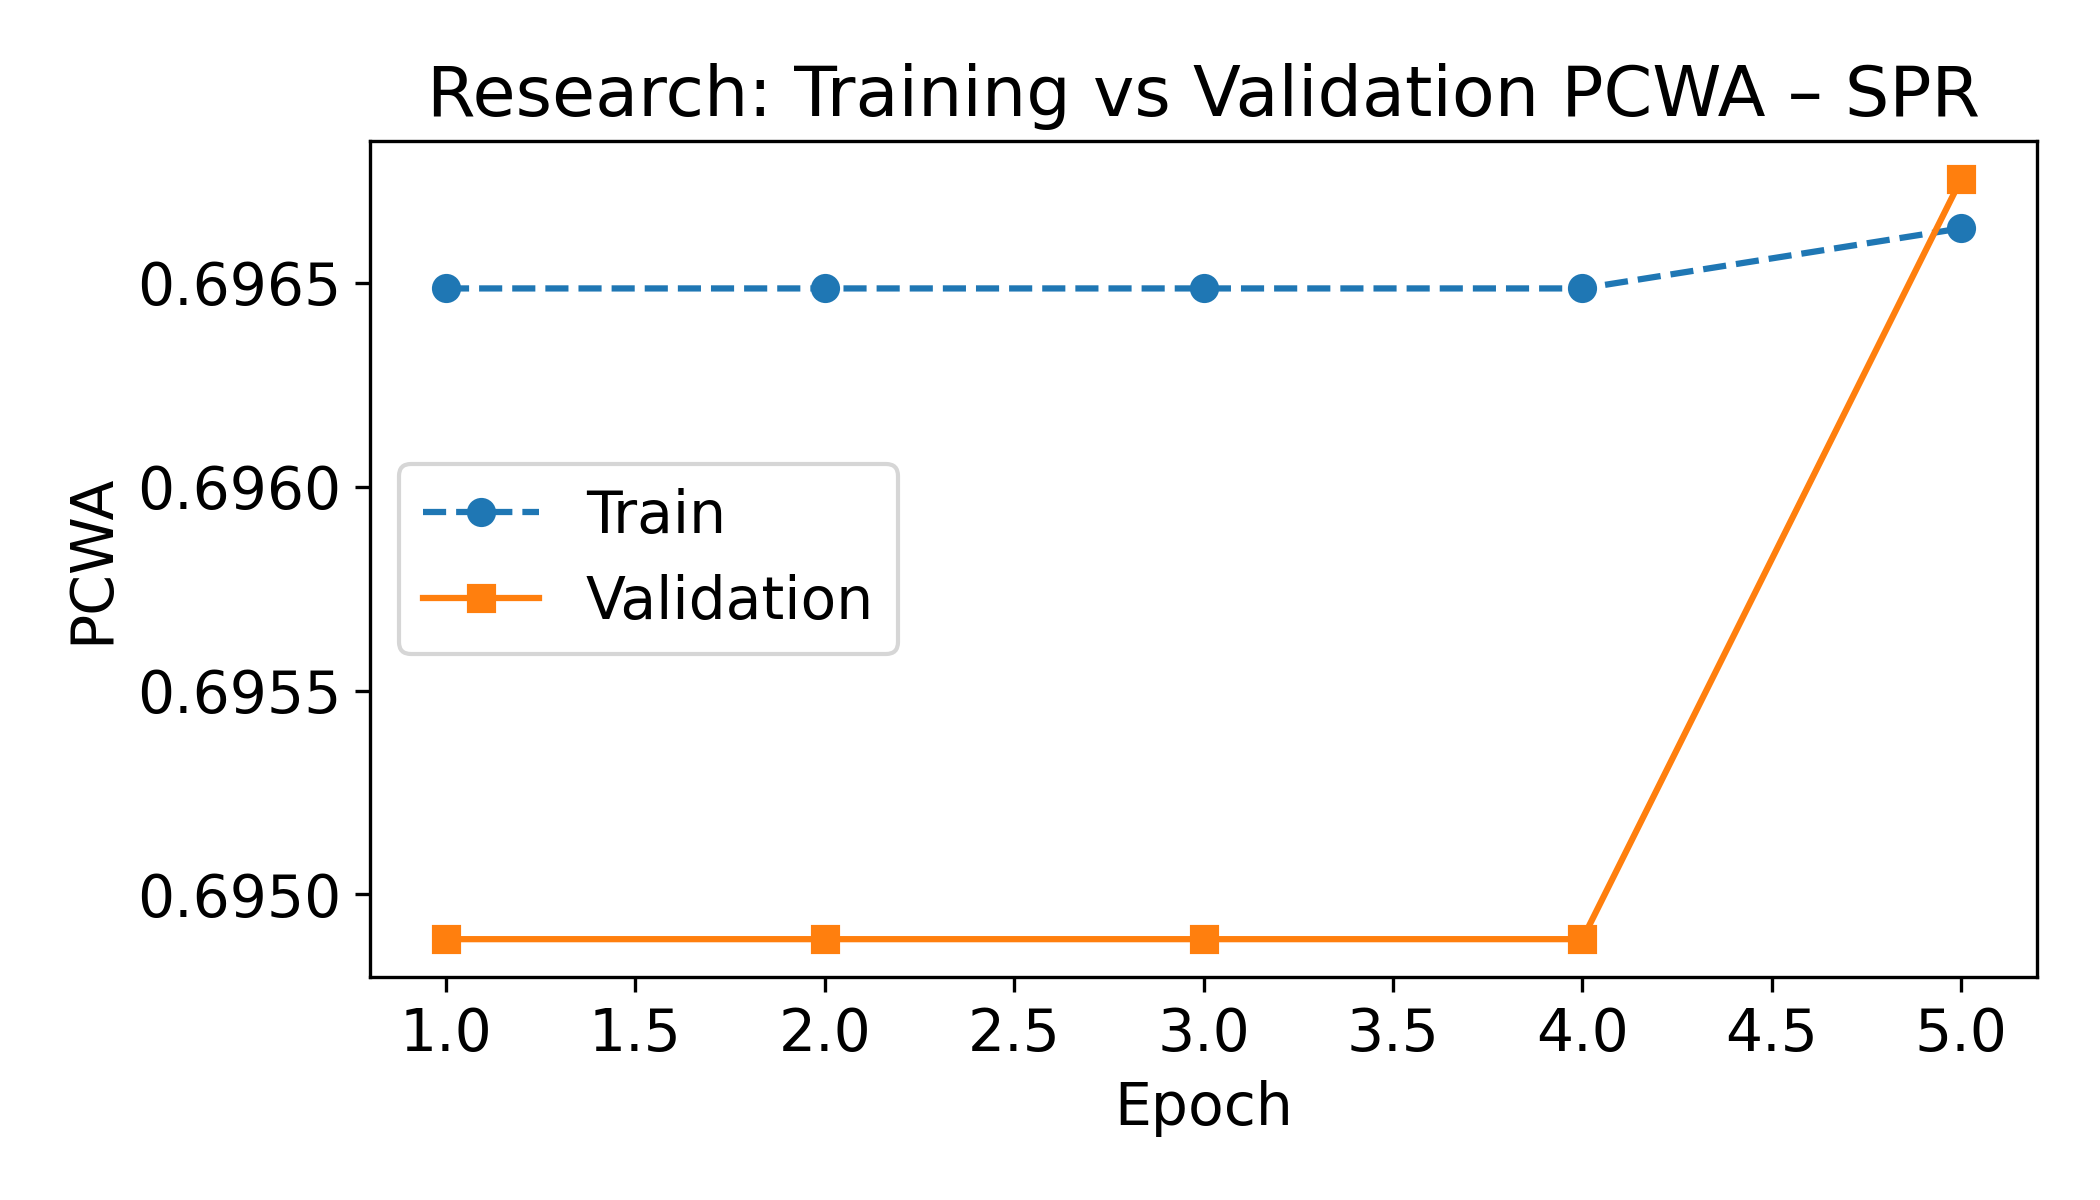
\includegraphics[width=0.46\textwidth]{Research_PCWA_Curves.png}}
\caption{Refined GNN architecture with PCWA. Deeper drops in training loss were observed, but the improvement did not generalize, indicating potential overfitting.}
\label{fig:research}
\end{figure}

\section{Conclusion}
Our findings reveal surprising pitfalls when improving GNN architectures. Although advanced techniques show promise under controlled conditions, real-world data introduces noise and instability. Future work could refine pooling and class-weighting strategies, or adapt dynamic hyperparameter schedules to mitigate overfitting. We hope these insights will inform more robust GNN design and evaluation protocols.

\bibliographystyle{iclr2025_conference}
\bibliography{references}

\clearpage
\appendix
\section{Supplementary Material}
For completeness, we include additional ablation results. Figure \ref{fig:ablation} combines the multi-dataset metrics and first-node PCWA experiments into a single overview. The cross-split performance varied widely, confirming that naive architectural tweaks do not necessarily yield consistent improvements.

\begin{figure}[ht]
\centering
\subfigure[Multi-Dataset Metrics]{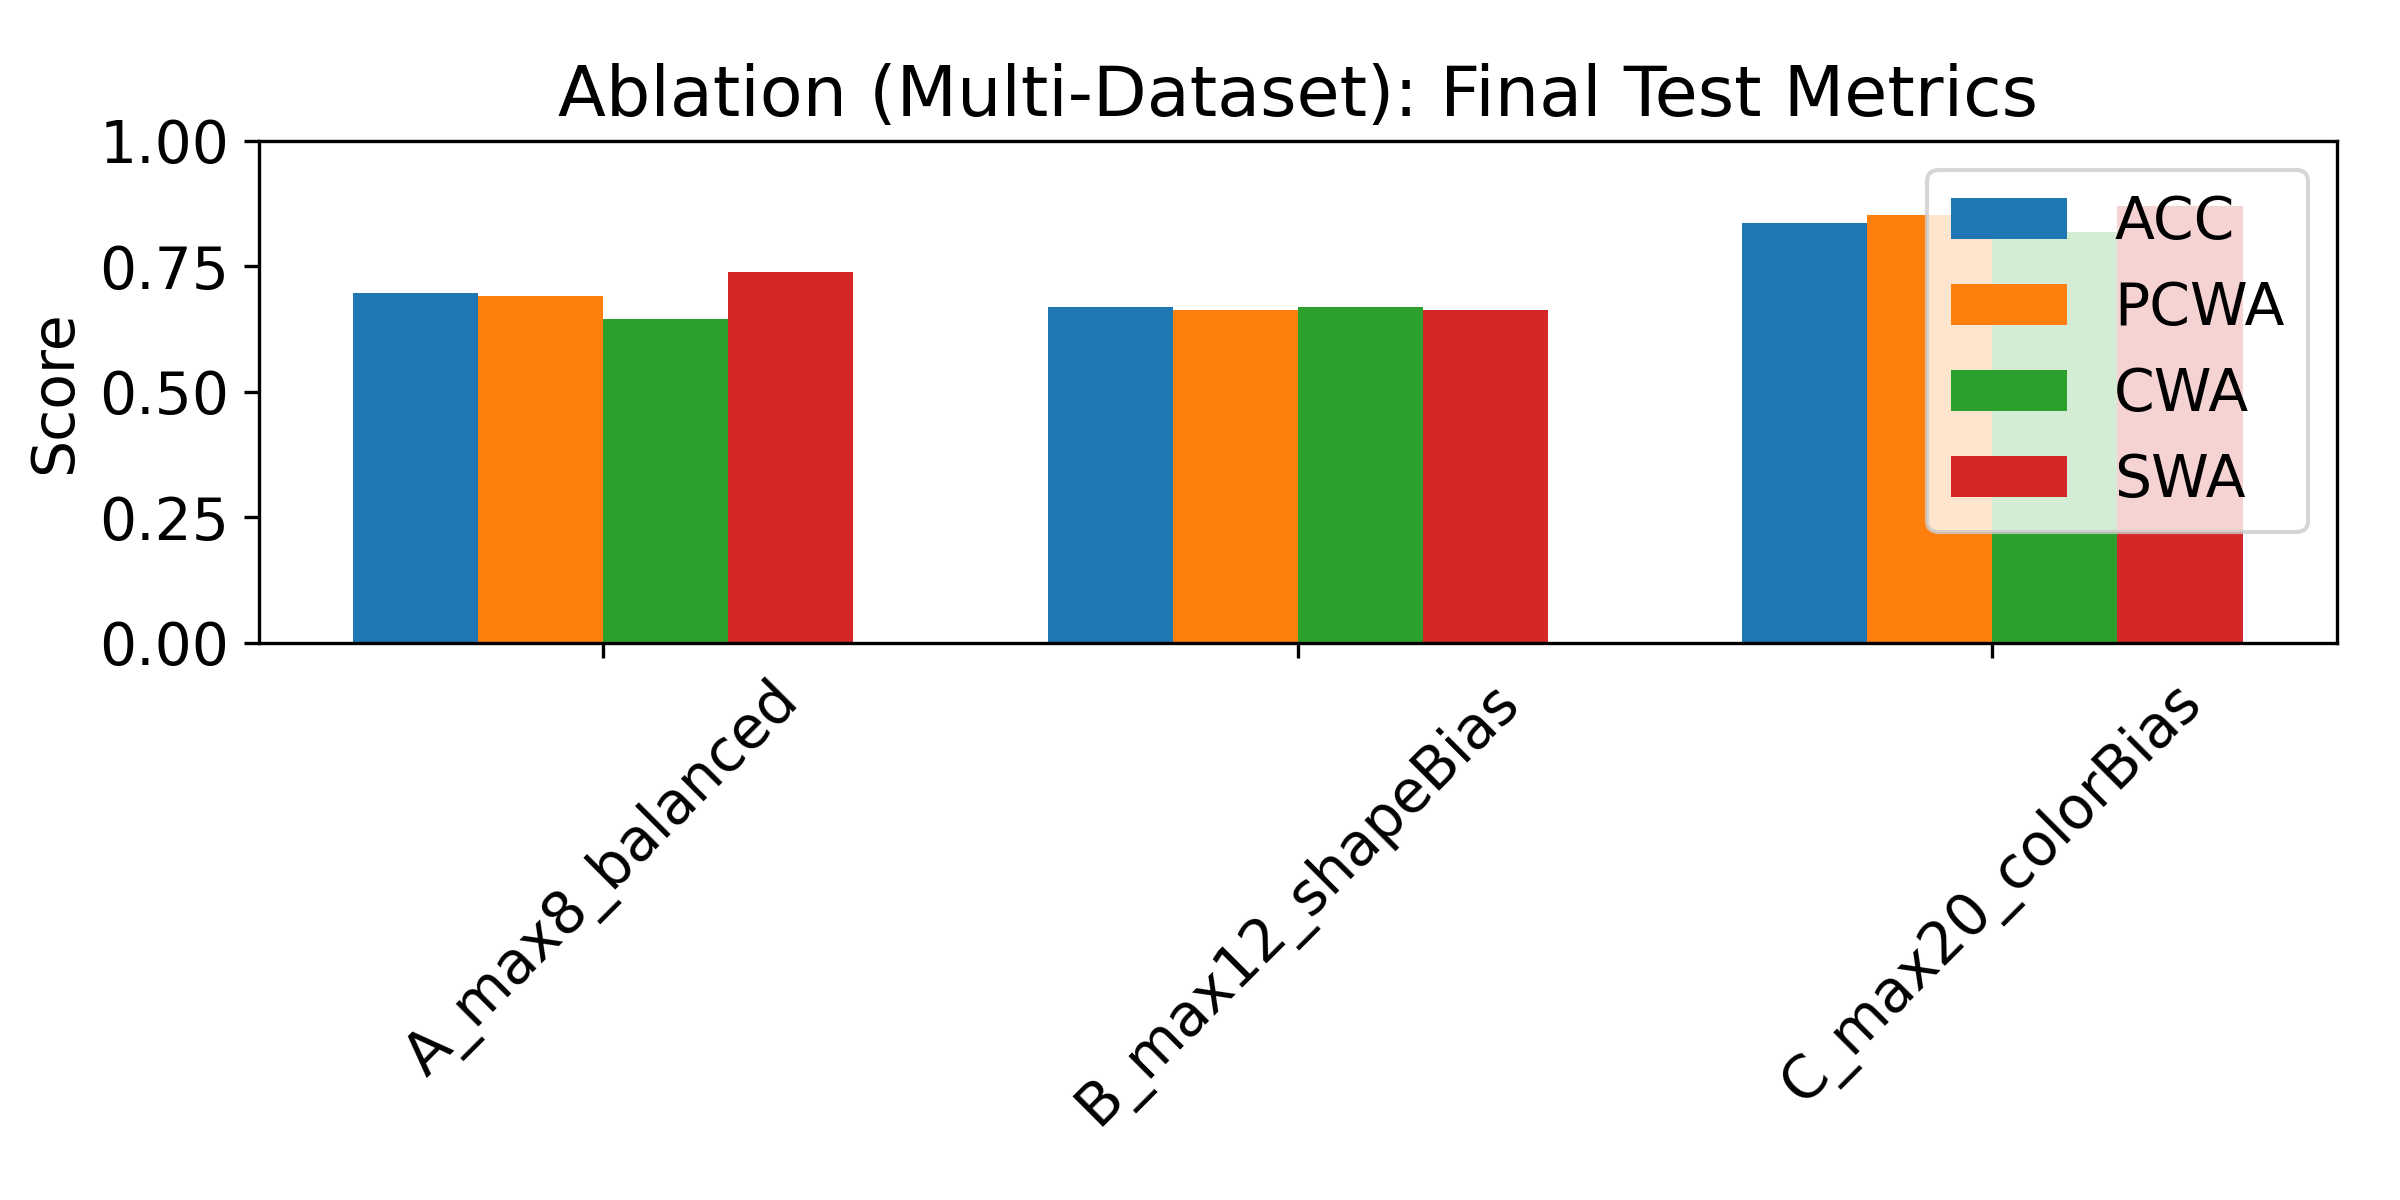
\includegraphics[width=0.46\textwidth]{Ablation_MultiDataset_Test_Metrics.png}}
\hfill
\subfigure[First-Node PCWA]{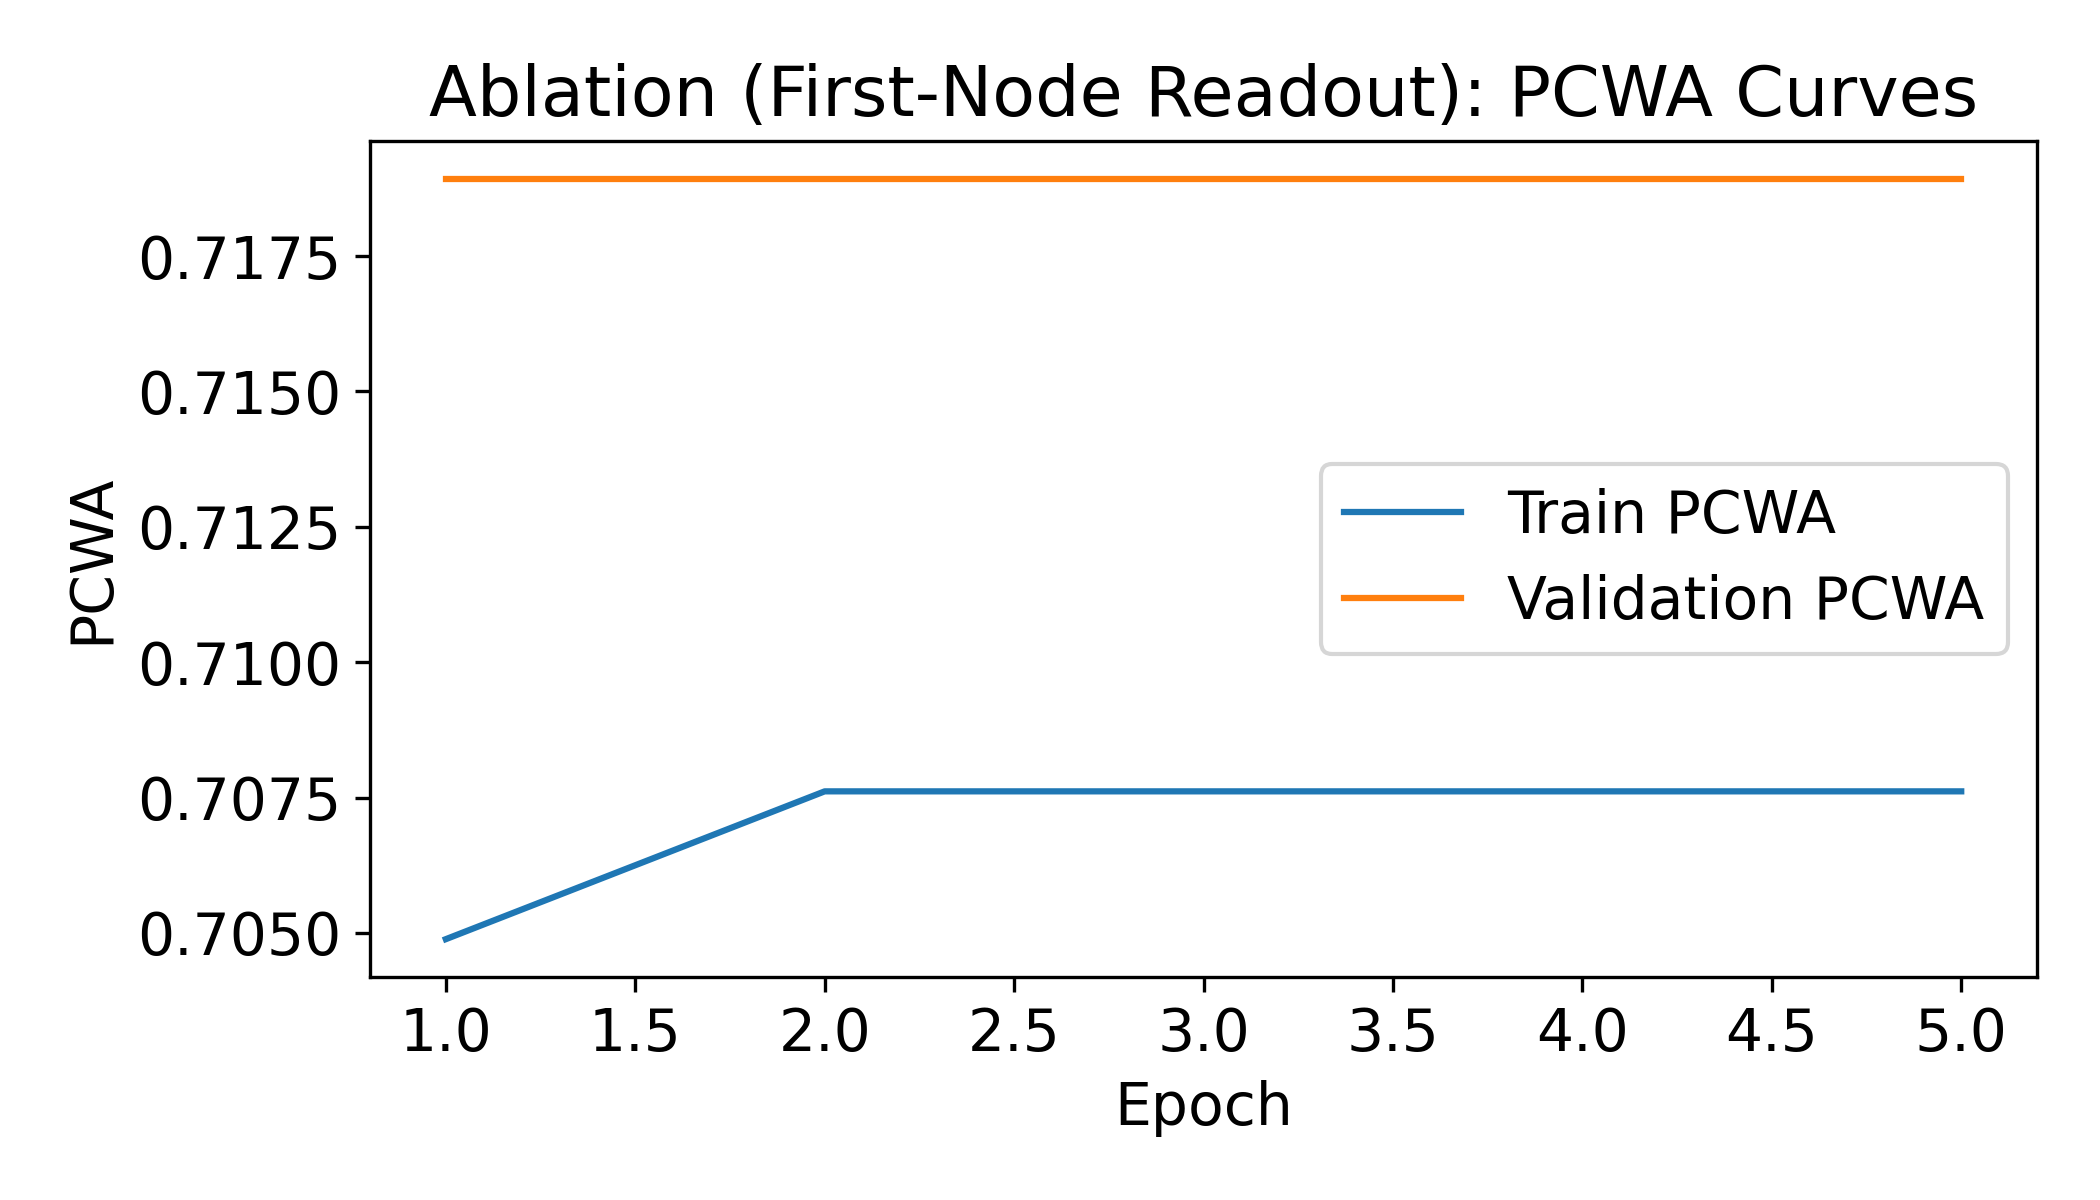
\includegraphics[width=0.46\textwidth]{Ablation_FirstNode_PCWA.png}}
\caption{Ablation studies. Subfigure (a) shows variability across different splits. Subfigure (b) demonstrates how restricting readout to the first node further inflates variance.}
\label{fig:ablation}
\end{figure}

\end{document}